\section{Question 2}
Data of the question:
$$
\mathrm{I}_x = 8_{kg.m^2},\quad \mathrm{I}_y = 10_{kg.m^2},\quad \mathrm{I}_z = 14_{kg.m^2}
$$
$$
\boldsymbol{\mathrm{q}}(0) = \begin{bmatrix}
    0.3 & 0.2 & 0.5 & 0.7874
\end{bmatrix}^T
$$

$$
\boldsymbol{\mathrm{\omega}}(0) = \begin{bmatrix}
    2 & 3 & -5
\end{bmatrix}^T \times 10^{-3}_{rps} = \begin{bmatrix}
    2\times 2\pi & 3\times 2\pi & -5\times 2\pi
\end{bmatrix}^T \times 10^{-3}_{rad/\sec}
$$

\section{part a}
Used MATLAB function(quat2eul) to calculate initial euler angles.
$$
\begin{bmatrix}
    \phi\\
    \theta\\
    \psi 
\end{bmatrix} = \begin{bmatrix}
  \ang{137.74}\\
  \ang{-0.86}\\
  \ang{65.16}
\end{bmatrix}
$$

\section{part b}
Equation of motion with gravity gradient:

\begin{align}
    I_x \dot\omega_x +  \omega_y \omega_z(I_z - I_y) = G_x\\
    I_y \dot\omega_y +  \omega_x \omega_z(I_x - I_z) = G_y\\
    I_z \dot\omega_z +  \omega_x \omega_y(I_y - I_x) = G_z\\
\end{align}

$$
\dot \omega_x = (G_x + \omega_y \omega_z(I_y - I_z))/I_x
$$

$$
\dot \omega_y = (G_y + \omega_x \omega_z(I_z - I_x))/I_y
$$

$$
\dot \omega_z = (G_z + \omega_y \omega_x(I_x - I_y))/I_z
$$

\begin{equation}
    \begin{bmatrix}
        \dot \omega_x \\
        \dot \omega_y \\
        \dot \omega_z
    \end{bmatrix} = \begin{bmatrix}
        p \\
        q \\
        r
    \end{bmatrix}  + \boldsymbol{\mathrm{C}}_R^b \begin{bmatrix}
        0 \\ -\omega_0 \\ 0
    \end{bmatrix} \to \begin{bmatrix}
        p \\
        q \\
        r
    \end{bmatrix} = \begin{bmatrix}
        \dot \omega_x \\
        \dot \omega_y \\
        \dot \omega_z
    \end{bmatrix} + \boldsymbol{\mathrm{C}}_R^b \begin{bmatrix}
        0 \\ \omega_0 \\ 0
    \end{bmatrix}
\end{equation}
where $\boldsymbol{\mathrm{C}}_R^b$ is transformation matrix.

\begin{equation}
    \boldsymbol{\mathrm{C}}_b^R = \begin{bmatrix}
        \cos(\theta)\cos(\psi) & -\cos(\phi)\sin(\psi) + \sin(\phi)\sin(\theta)\cos(\psi) & \sin(\phi)\sin(\psi) + \cos(\phi)\sin(\theta)\cos(\psi) \\
        \cos(\theta)\sin(\psi) & \cos(\phi)\cos(\psi) + \sin(\phi)\sin(\theta)\sin(\psi) & -\sin(\phi)\cos(\psi) + \cos(\phi)\sin(\theta)\sin(\psi) \\
        -\sin(\theta) & \sin(\phi)\cos(\theta) & \cos(\phi)\cos(\theta)
    \end{bmatrix}
\end{equation}


Using euler propagation:

\begin{equation}
    \begin{bmatrix}
        \dot \phi \\
        \dot \theta \\
        \dot \psi
    \end{bmatrix} = \begin{bmatrix}
        1 & \sin(\phi)\tan(\theta) & \cos(\phi)\tan(\theta)\\
        0 & \cos(\phi) & -\sin(\phi) \\
        0 & \dfrac{(\phi)}{\cos(\theta)} & \dfrac{\cos(\phi)}{\cos(\theta)}
    \end{bmatrix} \begin{bmatrix}
        p \\q \\ r
    \end{bmatrix}
\end{equation}

In linearized equation of motion we assume:

\begin{equation}
    \boldsymbol{\mathrm{C}}_b^R = \begin{bmatrix}
        1 & -\psi & \theta \\
        \psi & 1 & -\phi \\
        -\theta & \phi & 1
    \end{bmatrix}, \quad \begin{bmatrix}
        p \\ q \\ r
    \end{bmatrix} = \begin{bmatrix}
        \dot \phi \\
        \dot \theta \\
        \dot \psi
    \end{bmatrix}
\end{equation}

For the transformation from reference to body use the transpose of the desciberd matrix above.


The equations of motions solved in MATLAB with ode45 function. Below is the figure of euler angles simulation in 50 and 1000 seconds.

\begin{figure}[H]
    \caption{simulation of $\phi$ for 50 seconds}
    \centering
    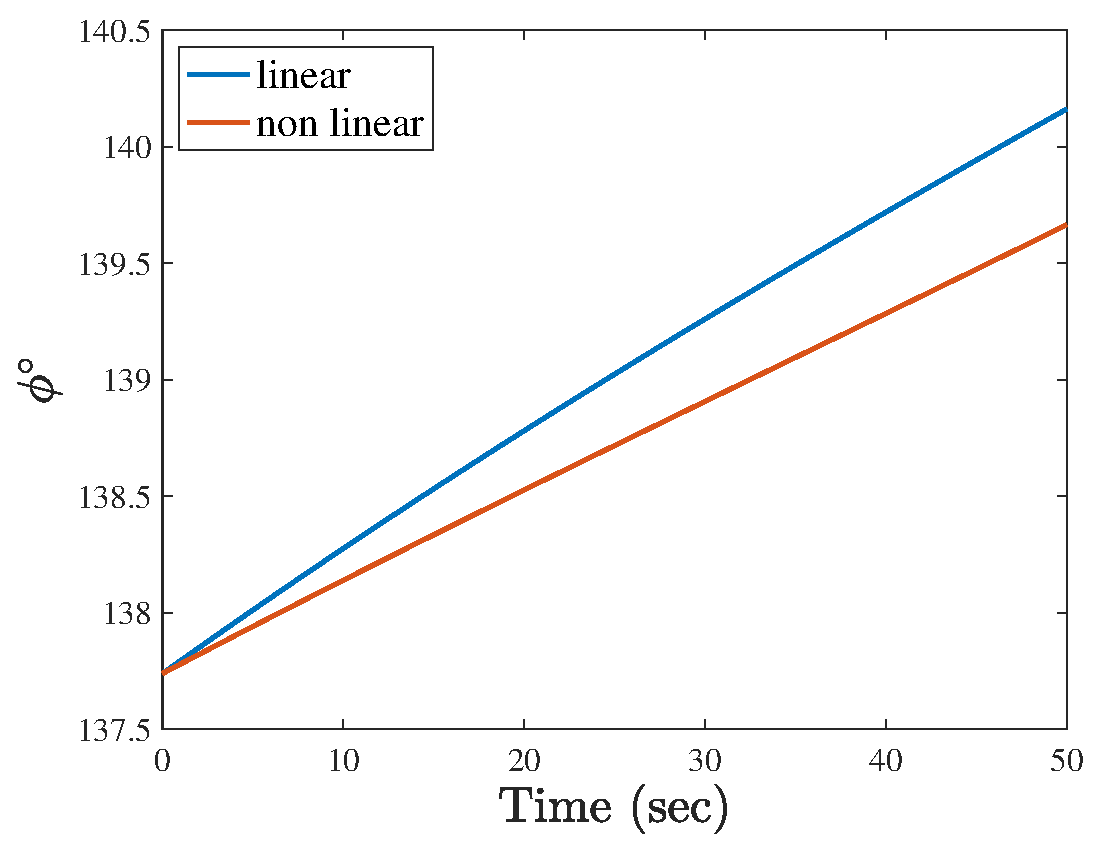
\includegraphics[width=12cm]{../Figure/Q2/phi_50}
\end{figure}

\begin{figure}[H]
    \caption{simulation of $\theta$ for 50 seconds}
    \centering
    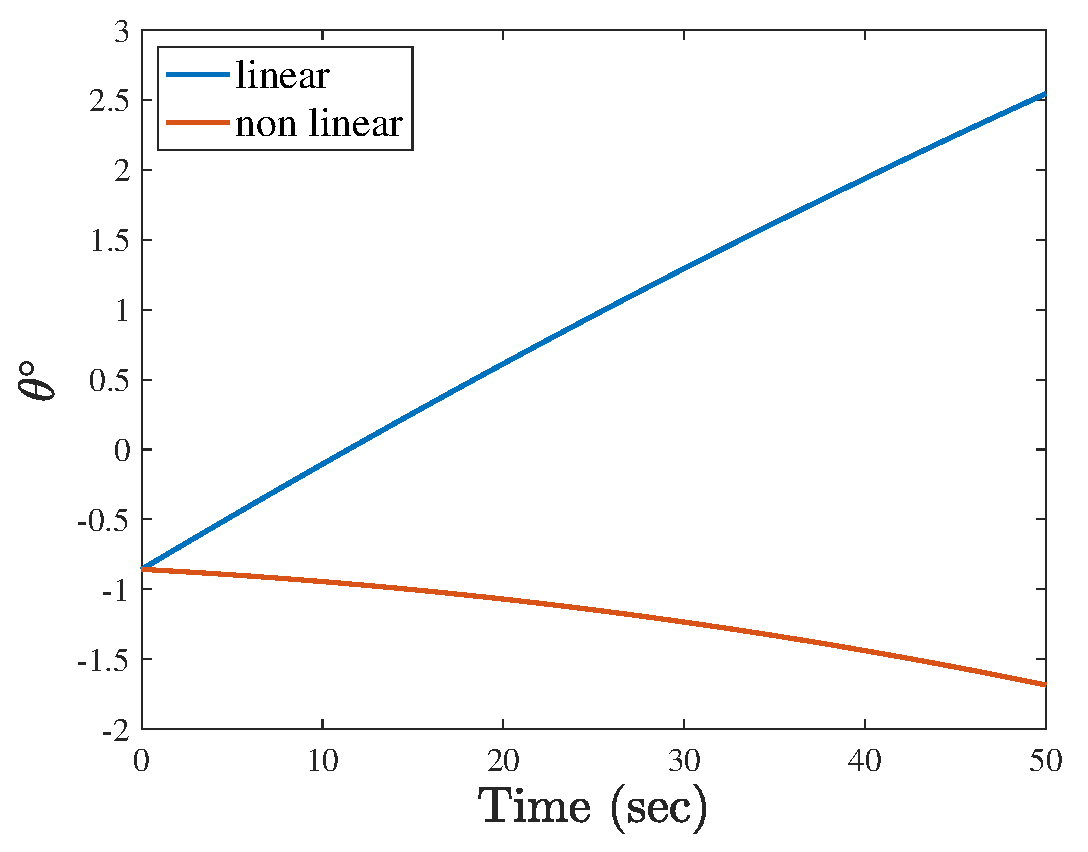
\includegraphics[width=12cm]{../Figure/Q2/theta_50}
\end{figure}

\begin{figure}[H]
    \caption{simulation of $\psi$ for 50 seconds}
    \centering
    \includegraphics[width=12cm]{../Figure/Q2/psi_50}
\end{figure}

%%%%%%%%%% 1000 %%%%%%%%%%
\begin{figure}[H]
    \caption{simulation of $\phi$ for 1000 seconds}
    \centering
    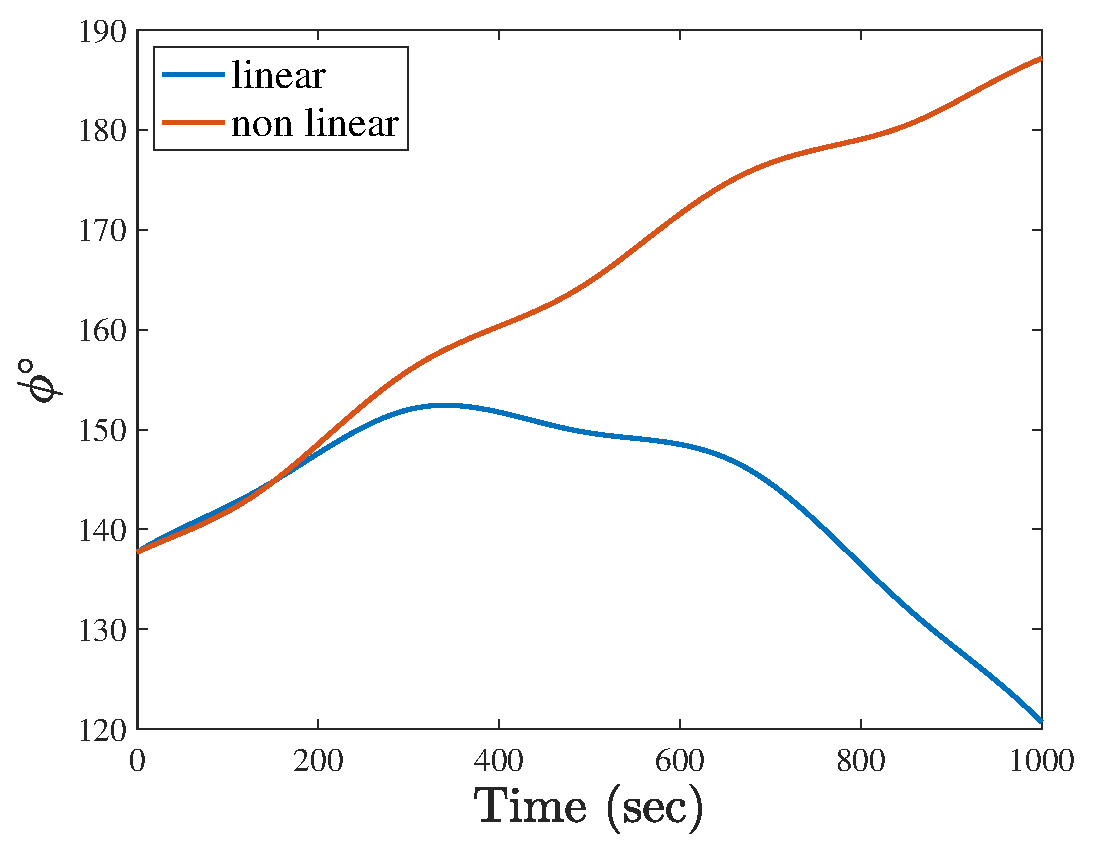
\includegraphics[width=12cm]{../Figure/Q2/phi_1000}
\end{figure}

\begin{figure}[H]
    \caption{simulation of $\theta$ for 1000 seconds}
    \centering
    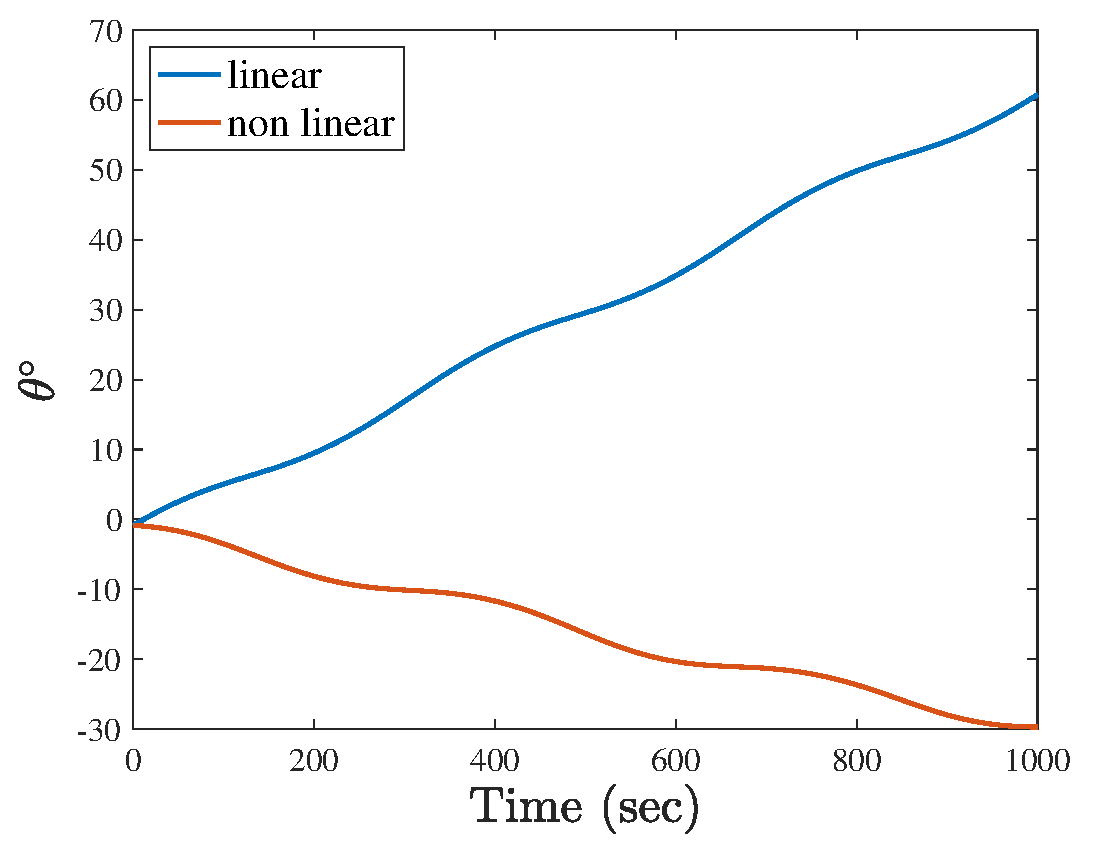
\includegraphics[width=12cm]{../Figure/Q2/theta_1000}
\end{figure}

\begin{figure}[H]
    \caption{simulation of $\psi$ for 1000 seconds}
    \centering
    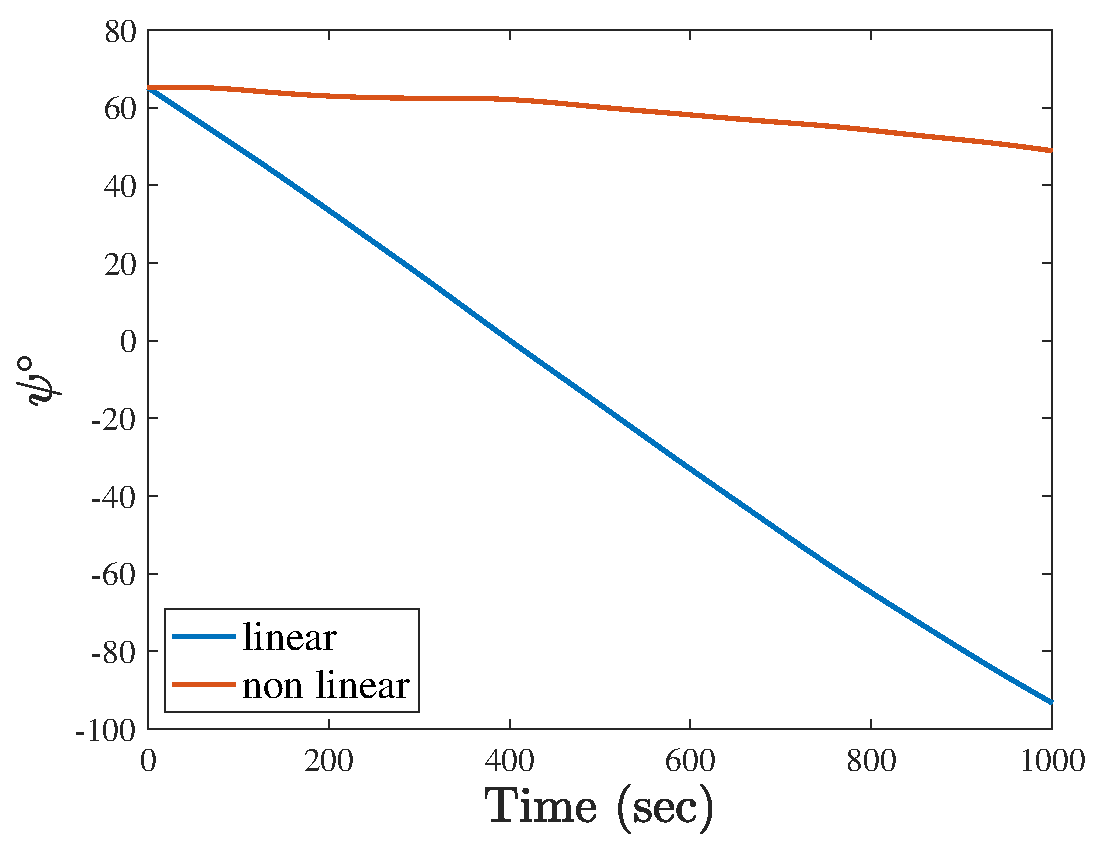
\includegraphics[width=12cm]{../Figure/Q2/psi_1000}
\end{figure}

\section{part d}

Used above equation with different initial conditions and add initial torque disturbance.

\begin{figure}[H]
    \caption{simulation of $\phi$ with torque disturbance}
    \centering
    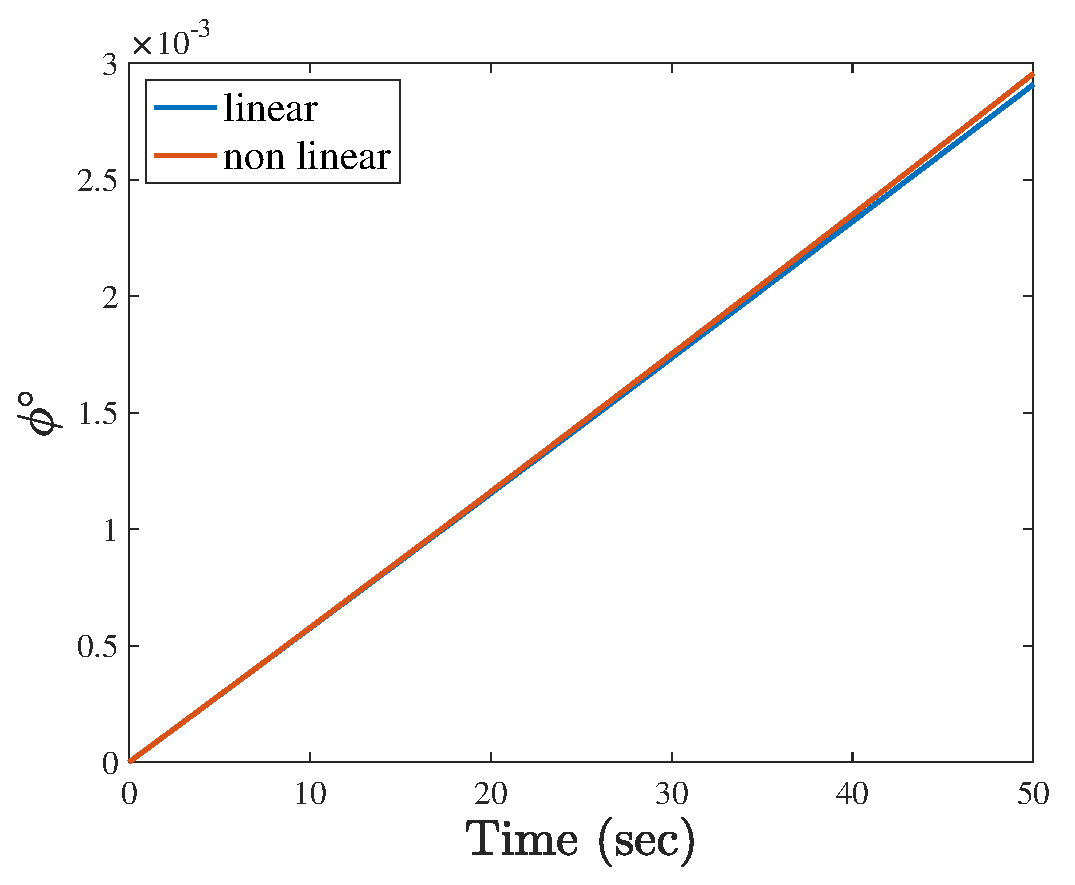
\includegraphics[width=12cm]{../Figure/Q2/phi_part_d}
\end{figure}

\begin{figure}[H]
    \caption{simulation of $\theta$ with torque disturbance}
    \centering
    \includegraphics[width=12cm]{../Figure/Q2/theta_part_d}
\end{figure}

\begin{figure}[H]
    \caption{simulation of $\psi$ with torque disturbance}
    \centering
    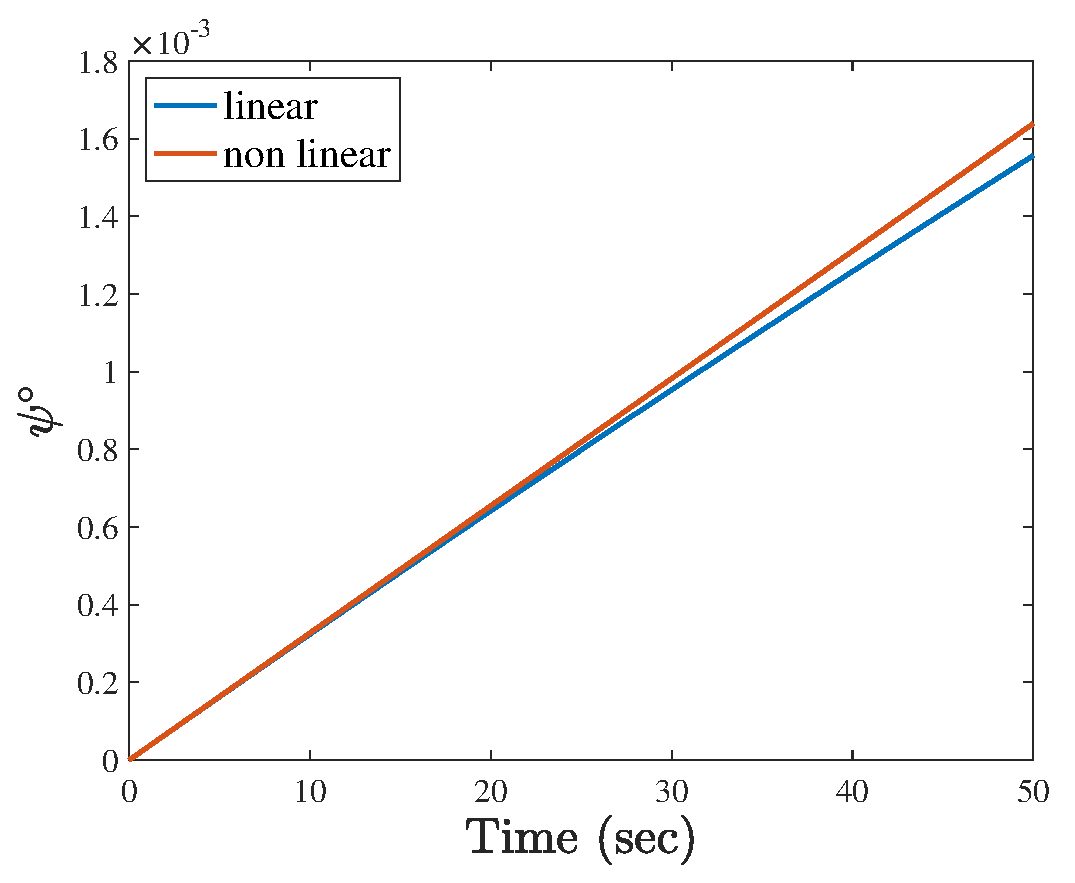
\includegraphics[width=12cm]{../Figure/Q2/psi_part_d}
\end{figure}
